%% This file is part of the UNRAVE Project 
%% Copyright 2016 the authors.  All rights reserved.


%% TODO:
%% Co-authors: Look for \stub{}s. If you can expand it, do so!

\documentclass[preprint,trackchanges]{aastex}

\usepackage{amsmath}
\usepackage{bm}

% This section can be removed at submission.
% ------------------------------------------
\usepackage{color}
\usepackage{datenumber}

\newcounter{dateone}
\newcounter{datetwo}

\newcommand{\difftoday}[3]{%
  \setmydatenumber{dateone}{\the\year}{\the\month}{\the\day}%
  \setmydatenumber{datetwo}{#1}{#2}{#3}%
  \addtocounter{datetwo}{-\thedateone}%
  \the\numexpr(\thedatetwo)\relax\space days
}
% ------------------------------------------

\IfFileExists{vc.tex}{\input{vc.tex}}{\newcommand{\githash}{UNKNOWN}\newcommand{\giturl}{UNKNOWN}}

\newcommand{\acronym}[1]{{\small{#1}}}

\newcommand{\project}[1]{\textsl{#1}}
\newcommand{\gaia}{\project{Gaia}}
\newcommand{\thecannon}{\project{The~Cannon}}
\newcommand{\rave}{\project{\acronym{RAVE}}}
\newcommand{\galah}{\project{\acronym{GALAH}}}
\newcommand{\ges}{\project{Gaia-ESO}}
\newcommand{\apogee}{\project{\acronym{APOGEE}}}
\newcommand{\aspcap}{\project{\acronym{ASPCAP}}}
\newcommand{\lamost}{\project{\acronym{LAMOST}}}
\newcommand{\hipparcos}{\project{Hipparcos}}
\newcommand{\epic}{\project{K2/EPIC}}

\newcommand{\stub}[1]{\textbf{#1}}

\newcommand{\teff}{T_{\mathrm{eff}}}
\newcommand{\logg}{\log g}

\newcommand{\Nstars}{483,330}

\newcommand{\argmin}[1]{\underset{#1}{\operatorname{argmin}}\,}


%\AuthorCallLimit=10


\begin{document}
% Remove at submission:
\slugcomment{{\color{red} \textbf{To appear on arXiv on 9 September 2016 (\difftoday{2016}{9}{7}away)}}}


\title{The \project{unRAVE} catalog}

\author{Andrew R. Casey}
\affil{Institute of Astronomy, Madingley Road, Cambridge CB3 0HA}

% Specific contributors to this work:
% There is some order already in mind, but final order will be determined by  contribution.
\author{Some combination of: Harry Enke, Gerry Gilmore, Keith Hawkins, David W. Hogg, Georges Kordopatis, Gal Matijevic, Melissa Ness, Jason Sanders, Matthias Steinmetz, Hans Walter-Rix}

% RAVE DR5 core team:
\author{Luca Casagrande, Cristina Chiappini, Andrea Kunder, Paul McMillan, Alessandro Siviero, Marica Valentini, Jennifer Wojno, Toma{\^z} Zwitter}

\author{and the \rave\ collaboration}


% Stubs for discussion & analysis.
% TODO: Inserting 2MASS photometry as fake pixels
% TODO: Censoring masks on abundance labels
% TODO: Priors on astrophysical parameters from isochrones
% TODO: Include velocities and rotational velocities at test time?


\begin{abstract}
The Milky Way may be our greatest laboratory for understanding galaxy formation.
This premise relies on the ability to precisely determine the astrometry and
chemistry for many individual stars, and to use those data to make inferences
about the Galaxy's formation and evolution. On 14 September 2016 the \gaia\ 
mission will release precise astrometry for $\approx2\times10^6$ stars.  
However, a comprehensive catalog of detailed chemical abundances to complement
those data is currently lacking.  The RAdial Velocity Experiment (\rave) survey 
has acquired spectra for 292,036 stars in common with the first \gaia\ data 
release, constituting the largest overlap of any stellar spectroscopic sample.  
Here we perform an independent analysis of \rave\ spectra using an implementation
of \thecannon\ that uses prior probabilities on atomic line formation and stellar
astrophysical parameters.  Our approach yields precise stellar labels at lower 
S/N ratios than most \emph{ab initio} approaches, allowing us to deliver improved
radial velocities, effective temperature $\teff$, surface gravity $\logg$, and 
chemical abundances of up to seven elements (Mg, Al, Si, Ca, Ti, Fe, Ni) for 
\Nstars\ stars.  We validate our results internally from repeat visits, and 
externally against existing high-resolution spectroscopic surveys.  The typical
precision in chemical abundances is X.XX~dex.  We provide spectrophotometric 
distances based on our labels, improving upon the parallax distances available
for the fainter targets in the first \gaia\ data release. \stub{A one-line 
science result based on RAVE/Hipparcos overlap}
\end{abstract}

\keywords{}

\section{Introduction} 
\label{sec:introduction}

The Milky Way is considered to be the best laboratory for understanding galaxy
formation and evolution.  This premise hinges on the ability to precisely measure 
the astrometry and chemistry for (many) individual stars, and to use those data 
to infer the structure, kinematics, and chemical enrichment of the Galaxy 
\citep[e.g.,][]{Schlaufman_2009,Deason_2011,Ness_2012,Ness_2013a,Ness_2013b,
Casey_2012,Casey_2013,Casey_2014a,Casey_2014b,Bovy_2016}.  However, these 
quantities are not known for even 1\% of stars in the Milky Way.  Stellar 
distances are famously imprecise \citep[e.g.,][]{van_Leeuwen_2007,Jofre_2015,
Madler_2016}, proper motions can be plagued by unquantified systematics from 
the first epoch observations \citep[e.g.,][]{Casey_Schlaufman_2015}, and 
stellar spectroscopists frequently report significantly different chemical 
abundance patterns \citep{Smiljanic_2014}.  The impact these issues have on our
scientific inferences cannot be understated.  They limit our understanding on a
number of sub-fields in astrophysics, including the properties of exoplanet host
stars, the formation (and destruction) of stars and clusters, as well as the 
structure of the Galactic disk, to name a few.


These formed just some of the scientific drivers for the \gaia\ space telescope.
\gaia\ is primarily an astrometric mission, providing precise positions,
parallaxes and proper motions for more than $10^9$ stars in its final data
release in 2022.  While this is a sample size about three orders of magnitude 
larger than its predecessor \hipparcos, both astrometry and chemistry are 
required to fully characterize the formation and evolution of our Galaxy.  For
this reason \gaia\ will also provide radial velocities, stellar parameters and
chemical abundances for a subset of brighter stars.  While astrometry for bright
and nearby stars will be imminently available, chemical abundances from \gaia\ 
will not be available until later releases.  Until those abundances are available,
astronomers seeking to use chemistry and kinematic measurements are reliant on 
ground-based spectroscopic surveys in order to complement the available astrometry.


The first \project{Gaia} data release will include positions, proper motions, and 
parallaxes for approximately two million stars in the Tycho-2 \citep{Hog_2000} 
catalog \citep{Michalik_2015a,Michalik_2015b}.  After cross-matching all major 
stellar spectroscopic surveys\footnote{Specifically we cross-matched the Tycho-2
catalog against the \apogee\ \citep{Zasowski_2013}, \ges\
\citep{Gilmore_2012,Randich_2013}, \galah\ \citep{DeSilva_2015},
\lamost\ \citep{Cui_2012}, and \rave\ \citep{Steinmetz_2006} 
surveys}, we found the RAdial Velocity Experiment (hereafter \rave) survey to 
have the largest overlap with the first \gaia\ data release: 292,036 
stars.  We then used the \gaia\ universe model snapshot \citep{Robin_2012} to 
estimate the precision in parallax and proper motions that will be available in 
the first \gaia\ data release (DR1) for stars in those overlap samples. Comparing
the expected precision to what is currently available, we further found that the
\rave\ survey will benefit most from \gaia\ DR1.  The distances of 63\% of the 
\rave--\gaia\ DR1 overlap sample (182,862 stars) are expected to improve with 
the first \gaia\ data release, and 47\% of stars are likely to have better 
proper motions (137,211 stars).  This motivated us to examine what chemical 
abundance information was available for \rave, and to evaluate whether we could
enable new chemodynamic studies by contributing to this existing set of chemical
abundances.


We briefly describe the \rave\ data in Section~\ref{sec:data}, before explaining
our method in Section~\ref{sec:method}.  In Section~\ref{sec:validation}
we outline a number of validation experiments, including: internal sanity checks,
comparisons with literature samples, and investigations to ensure our results
are consistent with expectations from astrophysics.  We discuss these results in
Section~\ref{sec:discussion}, and in Section~\ref{sec:conclusion} we provide 
concluding remarks as well as a description of how to access our results electronically.


\section{Data}
\label{sec:data}


\rave\ is a magnitude-limited stellar spectroscopic survey of the (nearby) Milky Way,
principally designed to measure radial velocities for up to $10^6$ stars.
Observations were conducted on the 1.2~m UK Schmidt telescope at the Australian 
Astronomical Observatory\footnote{Formerly the Anglo-Australian Observatory} from 
2003--2013.  The large 5.7~degree field-of-view and robotic fibre positioner (6dF)
made for very efficient observing.  Spectra for up to 150 targets were simultaneously
acquired, and when observations concluded in April 2013, a total of 574,630 spectra
had been collected of 483,330 unique objects. 


The target selection for \rave\ is based on the $I$-band apparent magnitude,
$9 < I < 12$, with a weak $J - K_s > 0.5$ cut near the disk and bulge \citep{Wonjo_2016}.  
The $I$ band was selected because it overlaps with the wavelength range that \rave\ 
operates in:  8410--8795~\AA.  This setup includes the \ion{Ca}{2} near-infrared 
triplet, and a number of atomic transitions of light-, $\alpha$-, and Fe-peak elements.
The \ion{Ca}{2} near infrared triplet lines are dominated by pressure broadening, 
which makes them strong and therefore visible even in very low S/N data or 
metal-poor stars.  This spectral region is also very well-studied.  It is one of the
key setups used for the ground-based high-resolution \ges\ survey
\citep{Gilmore_2012,Randich_2013}, and the \rave\ resolution and wavelength
coverage is comparable to the Radial Velocity Spectrometer on board the \gaia\
space telescope \citep{Recio-Blanco_2016}.


The exposure times for \rave\ observations were optimised to obtain radial 
velocities for as many stars as possible.  Detailed chemical abundances were
always an important science goal of the survey, but this was a secondary objective.  
For this reason the distribution of S/N ratios in \rave\ spectra is considerably 
lower than other stellar spectroscopic surveys where chemical abundances are the 
primary motivation.  The \rave\ spectra have an effective resolution 
$\mathcal{R} \approx 7500$ and the distribution of S/N ratios peaks at 
$\approx$50~per~pixel$^{-1}$.  For comparison, the \galah\ survey 
\citep{DeSilva_2015} --- which was specifically constructed for detailed chemical 
abundance analyses --- includes a wavelength range about 2.5 times larger at 
resolution $\mathcal{R} \approx 28,000$, and yet the \galah\ project still 
targets for S/N $\gtrsim100$.


Despite the relatively low resolution and S/N of the spectra compared to other
surveys, the \rave\ data releases have demonstrated the team's enormous success 
in deriving radial velocities, stellar astrophysical parameters ($\teff$, $\logg$),
as well as individual chemical abundances \citep{Steinmetz_2006,Zwitter_2008,
Siebert_2011,Kordopatis_2013,Kunder_2016}.  In this work we make use of spectra
that has been reprocessed for the fifth \rave\ data release.  These re-processing
steps include: a detailed re-reduction of all the original data frames, with flux
variances propagated at every step; an updated continuum-normalization procedure;
as well as revised determinations of stellar radial velocities and morphological
classifications. At the end of this processing for each survey observation we are 
provided with: rest-frame wavelengths, continuum-normalized fluxes, fractional 
uncertainties in continuum-normalized flux values, as well as relevant metadata.  
We refer the reader to the official fifth data release paper of the \rave\ survey, 
as presented by \citet{Kunder_2016}, for more details of this re-processing.


Given the high-quality of the normalization performed by the \rave\ team, we chose
not to re-normalize the spectra.  Our tests demonstrated that the procedure 
outlined in \citet{Kunder_2016} is sufficient for our analysis procedure. Therefore,
there is a limited number of pre-processing steps that we conducted before our
analysis could begin.  Firstly, we calculated inverse variance arrays from the
fractional uncertainties provided, then re-sampled the flux and inverse variance
arrays onto a common rest-wavelength map for all stars.  Depending on the fibre 
used and the stellar radial velocity, the range of rest-frame wavelength values
varied for each star.  Given that fluxes were unavailable in the edge pixels for 
most stars, we excluded pixels outside of the rest wavelength range 
$8423.2\,{\rm \AA} \le \lambda \le 8777.6\,{\rm \AA}$.  This corresponds to about
30~pixels excluded on either side of the common wavelength array, leaving us with
945~pixels per spectrum for science.


\section{Method}
\label{sec:method}

We chose to adopt a data-driven model --- rather than a physics-driven model ---
for this analysis.  Specifically we will use an implementation of \thecannon\
\citep{Ness_2015,Ness_2016}.  Although this choice complicated the construction 
of our model (e.g., see Section \ref{sec:the-training-set}), a data-driven model 
makes use of all available information in the spectrum and lowers the S/N ratio 
at which systematic effects begin to dominate.  In other words, a well-constructed
data-driven model will yield more precise labels (e.g., stellar parameters and
chemical abundances) at low S/N ratios than most physics-driven models\footnote{
However, see \citet{Casey_2016a}}.  This is particularly relevant for the 
low-resolution \rave\ data analysed here, because about half of the spectra have
S/N $\lesssim 50$. 


Throughout this work we adopt the assumptions and nomenclature first set out in
\citet{Ness_2015}, and extended in \citet{Casey_2016b}.  However, one distinction 
here with \citet{Casey_2016b} is that in this work the \emph{labelled} set and the
\emph{training} set will be the same set.  In \citet{Casey_2016b} two subsets of
the labelled set were defined: the training set and a distinct validation set.
This allowing us to train on the \emph{training set} and then test on the 
\emph{validation set}.  However in this work the labelled set is relatively 
small, about an order of magnitude smaller than what was available in 
\citet{Casey_2016b}, and therefore no validation set exists. We will use all 
labelled set stars in the training step and supplement our validation experiments 
with literature comparisons.  Thus, throughout this work we will use the terms 
\emph{labelled set} and \emph{training set} interchangeably.  Below we describe 
how we constructed the training set, before we outline the model that we adopt.


\subsection{The training set}
\label{sec:the-training-set}

We sought to construct a training set consisting of stars across the main-sequence,
sub-giant, and the red giant branch.  We required stars with precisely measured
effective temperature $\teff$, surface gravity $\logg$, and elemental abundances
of Fe, Mg, Si, Ti, Ca, Al, and Ni.  This proved to be difficult because the magnitude
range of \rave\ does not overlap substantially with high-resolution spectroscopic
surveys.  The fourth internal data release of the \ges\ survey includes 
giant and main-sequence stars, but only 142 overlap with \rave.  The most recent 
\apogee\ data release \citep{sloan_dr13} reports labels for stars on the
giant branch and (uncalibrated values for) the main-sequence, but our tests indicated
that the main-sequence labels suffered from significant systematic effects.  A flat, 
then `up-turning' main-sequence is present, and the metallicity gradient trends in 
the opposite direction with respect to $\logg$ on the main-sequence (i.e., metal-poor
stars incorrectly sit above the isochrones in a classical Hertzsprung-Russell diagram)
If we consider lower-resolution studies, there are 2,369 stars that overlap with 
\lamost\ --- of which 2,213 have positive S/N ratios in the $g$-band 
(\texttt{snrg}).  However, the labels are expectedly less precise given the lower 
resolution, no detailed abundance information is available for main-sequence stars
\footnote{Abundance information is available for \lamost\ stars from \citet{Ho_2016},
but that sample contains only giant stars}, and similar systematic trends are apparent
in the lower main-sequence.  The \galah\ survey has a good overlap with \rave, but 
results from that sample are not yet precise enough for our purposes.


These constraints forced us to construct a heterogeneous training set.  Given previous
successes in transferring high S/N ratio labels from \apogee\ \citep{Ness_2015,
Ness_2016,Ho_2016,Casey_2016b}, we chose to use the 1,355 stars in the \apogee---\rave\ 
overlap sample for giant star labels in the training set.  Of these, about 900 are 
giants according to \apogee.  From this sample we selected stars to have: metallicity
determinations ([Fe/H] $> -5$); high S/N ratios in both the \apogee\ and \rave\ spectra
($>200$ in \apogee; $>50$ in \rave); and we further required that the \aspcap\ pipeline 
did not report any peculiar flags (\texttt{ASPCAPFLAG = 0}).  These restrictions left 
us with 357 stars along the giant branch, with metallicities ranging from 
$[{\rm Fe/H}] = -1.62$ to 0.32.  Intermediate tests with globular cluster members showed
that the metallicity range of the training set needed to extend below 
$[{\rm Fe/H}] \lesssim -2$ in order for our catalog to be practically useful.
Therefore, as we will describe in more detail below, we supplemented this sample with 
giant stars from the \epic\ catalog \citep{Huber_2016}.


Assembling a training set for the main-sequence and sub-giant branch was more complex.
There are no spectroscopic studies that have a large enough sample size that overlap 
with \rave, and which also cover our required range in stellar parameters 
(e.g., FGKM-type stars).  Moreover, most of the spectroscopic studies we considered 
exhibit a flat lower main-sequence, a systematic consequence of the analysis method 
adopted \citep[e.g., see][for a discussion]{Bensby_2014}.  For these reasons we chose
to make use of the \epic\ catalog \citep{Huber_2016} for the training set labels on
the main-sequence and sub-giant branch.  The \epic\ catalog follows from the successful
\project{Kepler} input catalog \citep{Brown_2011}, and provides probabilistic stellar 
classifications for 138,600 stars in the \project{K2} fields based on the 
astrometric, asteroseismic, photometric, and spectroscopic information available for
every star.  There are 4,611 stars that overlap between \epic\ and \rave.


\epic\ differs from the \project{Kepler} input catalog because \epic\ does not 
benefit from having narrow-band $DDO_{51}$ photometry in order to aid dwarf/giant 
classification.  Despite this limitation the labels in the \epic\ catalog have 
already been shown to be accurate and trustworthy \citep{Huber_2016}.  However, 
when the posteriors are wide (i.e., the quoted confidence intervals are large) 
due to limited information available, it is possible that a star has been 
mis-classified.  This is most prevalent for sub-giants, where \citet{Huber_2016} 
note that $\approx55-70$\% of sub-giants are misclassified as dwarfs.  The 
probability of misclassification is usually quantified in the uncertainties of 
each star; most sub-giants that could be dwarfs have large confidence intervals.  
Therefore, requiring low uncertainties will decrease the total sample size, but 
will remove most misclassifications.  The situation is far more favourable for 
dwarfs and giants.  Only $1-4$\% of giant stars are misclassified as dwarfs, and 
about 7\% of dwarfs are misclassified as giants.  To summarise, the \epic\ labels 
with narrow confidence intervals are usually of high fidelity, and any spurious 
misclassifications would be clearly distinguishable if spectra were available. 


We sought to have a small overlap between our giant and main-sequence star training
sets.  Most of our giant training set is encapsulated within $0 < \logg < 3.5$, 
however there is a sparse sampling of stars reaching to $\logg \approx 4$.  For
the \epic\ main-sequence/sub-giant star training set we required $\logg > 3.5$,
allowing for $\approx0.5$~dex of overlap between the two training sets.  We further
employed the following quality constraints: the upper and lower confidence intervals 
in $\teff$ must be below 150~K; the upper and lower confidence intervals in $\logg$ 
must be less than 0.15~dex; the $S/N$ of the \rave\ spectra must exceed 
30~per~pixel$^{-1}$; and $\teff \leqslant 6750$~K.  Unfortunately these strict constraints
removed most metal-poor stars, which we later found to cause the test labels to have
under-predicted abundances for dwarfs of low metallicity.  For this reason we relaxed
(ignored) those quality constraints for stars in the \epic\ catalog with 
$[{\rm Fe/H}] < -1$.  Of the stars we forcibly included with $[{\rm Fe/H}] < -1$,
none were classified as being sub-giants in \epic, therefore they have a low (7\%)
likelihood of misclassification.  After training a model based on main-sequence and
giant stars (Section \ref{sec:the-model}), we found we could further identify 
misclassifications by leave-one-out cross-validation (iteratively, even).  However,
we chose not to do this because the number of likely misclassifications in the training
set was negligible ($\approx1$\%), and the improvement in main-sequence test set labels
was minimal.  The distilled sample of the \rave--\epic\ overlap catalog contains 583 
stars (of 4,611).


We previously alluded to including giant stars from \epic\ in our training set based 
on \apogee\ labels.  This was principally to ensure an adequate balance of metal-poor
giant stars in the training set.  Without this inclusion, we again found that the
abundances of giant stars would be under-predicted at low metallicity, critically 
affecting any inferences we wish to make with low metallicity stars (e.g., globular
clusters).  The metallicities in the \epic\ catalog come from a variety of spectroscopic
sources, or photometrically-selected when no spectroscopic information is available.
While these heterogeneous metallicities may introduce scaling differences, on balance we
later found that it was more important to include reasonably accurate (albeit imprecise)
metallicities of metal-poor stars in the training set rather than excluding metal-poor
stars entirely.  In Section~\ref{sec:validation} we show that these potential issues
have a negligible impact on the test set labels, and we further show that our abundances
are consistent with high-resolution studies in the literature.


We have constructed a justified training set for stars across the main-sequence, sub-giant,
and red giant branch.  However the lack of overlap between \rave\ and other works have
resulted in a somewhat peculiar situation. Detailed abundances are available from \apogee\
for all giant stars in our sample, but only imprecise metallicities are available from
\epic\ for stars on the main-sequence and the sub-giant branch.  To our knowledge this 
problem has not been addressed with data-driven models in the astrophysics literature.
In the following section we will construct a simplified model that does not include detailed
abundances, before demonstrating how we (1) improve upon the imprecise metallicities for 
main-sequence/sub-giant stars, and (2) translate abundances from the giant branch stars 
to the main-sequence/sub-giant branch sample.


\subsection{The model}
\label{sec:the-model}


% Describe The Cannon basic model, vectorizer, etc.
% Fitting time errors, etc.



% Here we will first consider only a three parameter model.
% APOGEE used only quadratic model, worked for giants
% We experimented with a quadratic model only. 
% Useful for identifying mis-classifications but the structure wasn't all there..
% worked but didn't show the structure in detail.
% Split into two different models with partial overlap.
% One for giants and one for dwarfs.
% The labels for stars in the training sets are shown in Figure X.


% We trained all three models.
% Note the differences in metallicity scales.
% The K2/EPIC stuff is accurate but imprecise, whereas the APOGEE stuff is precise, usually precise (except Ti?)
% Look at spectral derivatives.
% Show the model internals are relatable.
% Map spectral derivatives from giant model to main-sequence model.
% Update the model with those new spectral derivatives.


% We ran all three models on all spectra.
% How we combined the results into one.
% Refer to test set HRD.


% Restricted to 3-label model, but the giant set includes abundance labels.
% The spectral range covered by \rave\ includes atomic transitions of X, Y, Z elements.
% The strongest lines are indicated in Figure XXX.


% Censoring masks
% Transfering coefficients, etc.

\section{Validation experiments}
\label{sec:validation}


\subsection{Internal validation}
We first conducted leave-one-out cross-validation to validate our results.
For each training set star we removed that star from the training set and
then re-trained the model.  Using that re-trained model, we then treated
the excluded star as a test star and compared our inferred labels to the
test set labels.  We show the results of this experiment in Figure
\ref{fig:loocv-comparison}.  The bias and root mean square (RMS) error in 
$\teff$ is XX~K and XX~K, and in $\logg$ is X.XX~dex and X.XX~dex,
respectively.  The bias in abundance labels is negligible --- between
X.XX to X.XX --- and the RMS varies from X.XX ([XX/H]) to X.XX ([XX/H]).
% Fill this in tomorrow.


The \rave\ survey performed repeat observations for 23,288 stars  with time 
intervals ranging from a few hours to up to four years.  This timing was 
constructed to be quasi-logarithmic such that spectroscopic binaries could
be optimally identified. Most of the stars that were observed multiple times
were only observed twice, with thirteen visits being the maximum number 
of observations for any target.  These repeat observations allow us to 
quantify the level of (in)correctness in our formal errors.  For every star
with multiple visits we constructed a high S/N stacked spectrum for that
star, weighted by the inverse variances in the individual visit spectra,
which then served as the basis of comparison to all individual visits.  
Figure \ref{fig:formal-errors-comparison} shows the difference in labels 
between the comparison spectrum and a repeat visit, normalized by their 
formal errors summed in quadrature (e.g., $\Delta\logg/\sqrt{\sigma_{\logg,stacked}^2 + \sigma_{\logg,visit}^2}$).
If our measurements were unbiased by S/N and the errors were representative, 
these values should be normally distributed with a zero mean and unit variance.
\stub{Are they? Should we inflate our formal errors?}


% Internal validation:
% --> bootstrap resampling of the training set?

% Identify outliers:
% --> Chi-sq of the sample.
% --> Convex hull? Distance to plane?
% --> Stars with morphological classification
% --> Some rogue gallery of a few high S/N cases that have clearly gone haywire?


\subsection{External validation}
\label{sec:external-validation}

Here we cross-match our results against literature samples to verify that
our labels are accurate.  Because this work is an independent analysis, our
first point of reference is against the official \rave\ data releases.  These
comparisons are shown in Figures \ref{fig:rave-dr4-comparison} and 
\ref{fig:rave-dr5-comparison}, where we show our labels with respect to the
results in the fourth and fifth \rave\ data releases, respectively.  In order
to provide a fair comparison, we only show stars that meet a number of quality
flags in both samples. 
\stub{What selections qualify as a fair comparison in both samples?}
There is very good agreement in $\teff$, with a bias
and RMS of just XX~K and XXX~K, respectively.  We find our $\logg$ values are
closest to the `calibrated' \rave\ surface gravities, which make use of 
asteroseismic information to correct (increase) the $\logg$ values along the
giant branch.  The calibrated \rave\ surface gravities also correct the 
location of the red clump (by $\sim0.5$~dex) to be in the same position in our
results.  However, while our $\logg$ values generally agree with the calibrated
\rave\ values along the giant branch, our $\logg$ values do differ slightly 
along the main-sequence.  This is principally because the main-sequence in 
this work tends to taper down towards higher $\logg$ values at cooler 
temperatures, whereas the comparison sample tend to have a slightly flatter
main-sequence.  This difference is not likely to have a very significant 
effect on the detailed abundance or spectrophotometric distance determinations
between these studies.

\stub{What abundances are available?}

% This is more relevant for the discussion, not description of the training set.
We note that the while Ti can be measured, its values in both 
APOGEE DR12 and DR13 are known to not follow the expected Galactic trends \citep{Holtzman_2015, Hawkins_2016}.

\stub{Any differences in RAVE abundances?}


% External validation: 
% --> Gaia-ESO Survey
% --> APOGEE / EPIC (whichever was not used)
% --> Literature studies presented in Kordopatis+ 2014
% --> Gold standards (incl. exoplanet host star studies): Reddy (2003, 2006), Bensby (2014), Valenti & Fischer (2005)

\subsection{Astrophysical validation}

After verifying that our stellar labels are comparable with other
high-resolution studies, here we verify that the abundance labels we find
are consistent with expectations from astrophysics.  One example is stars in
globular clusters, which show anti-correlations in light element abundances 
\citep[e.g.,][and references therein]{Da_Costa,Carretta_2009}. In the \rave\
survey, \cite{Anguiano_2015} found 70 stars with positions and radial velocities that are
consistent with being members of globular clusters.  We have used that sample
Specifically, this GC sample includes 49 stars belonging to NGC~5139 ($\omega$~Centauri), 11 members of the retrograde
globular cluster NGC~3201, and 10 members of NGC~362.  
\stub{Were any of these stars unintentionally in the training set? \\ KH: Not using my training sets.}
All of these systems are well-studied and exhibit abundance anti-correlations 
in Na--O and Mg--Al \citep{people}.  Other correlations are also present 
(e.g., C--N), but those relationships are less relevant for this work because 
we do not measure C and N abundances here.


We show the detailed abundances for these globular cluster members in
Figure \ref{fig:globular-cluster-abundances}.  For comparison purposes we
have included abundances from the high-resolution studies of \citep{people}.
\stub{What do we find?}

% Assuming we recover these relationships...
Indeed, this demonstrates that our abundance labels can be used to identify
globular cluster members that are now tidally disrupted \citep{Anguiano_2016,Kuzma_2016,Navin_2016},
even for stars with low S/N ratios.

% Some literature notes:
% See http://iopscience.iop.org/article/10.1088/0004-637X/731/1/64/pdf
% NGC 3201 has Na-O anti-correlation: Carretta et al. (2009)
% NGC 362 has "two discrete groups along the Na-O anti-correlation": https://arxiv.org/abs/1307.4085
% NGC 362 has Mg-Al relationship (low Mg scatter, large Al scatter) --> Carretta (2013)
% NGC 362 has a large metallicity spread in RAVE (Anguiano_2015) but not the case in high-res studies (e.g. https://arxiv.org/abs/1307.4085 has a metallicity spread of 0.05/0.08 dex) may indicate better cluster selection needed and can be done with cannon results.
% NGC 3201 has Mg-Al relationship (http://arxiv.org/pdf/1305.3645.pdf and references therein)



% Astrophysical validation:
% --> Residuals as a function of galactic position? (DIBS)



\section{Discussion}
\label{sec:discussion}





\section{Conclusion}
\label{sec:conclusion}

% We have introduced a non-parametric version of The Cannon that uses strict priors on line formation (censoring masks), and prior probability distributions on astrophysical parameters, using isochrones.
% We ran it on the entire RAVE spectra.
% We deliver effective temperature, surface gravity, and abundances of up to 8 elements for \Nstars.  Our internal and external validation tests suggest that we achieve a typical precision of X~K in $\teff$, 0.0X~dex in $\logg$, and $\approx{}X.XX$ in individual chemical abundances.  This catalog constitutes the largest collection of stellar abundances for stars in the first \project{Gaia} data release.  When combined with positions and 3D velocities from \project{Gaia}, the \project{UNRAVE} catalog will likely be crucial for understanding our local place in the Milky Way.


\subsection*{Access the results electronically}

% TODO: Replace ZENODO-URL with a data url
Source code for this project is available at \texttt{\giturl}.
This document was compiled from revision hash \texttt{\githash} in that repository.
Inferred labels and covariance matrices are available electronically with 
associated metadata at \texttt{\url{ZENODO-URL}} \citep{DATA_REPOSITORY}.  
Please note that it is a condition of using these results that the fifth \rave\ 
data release by \citet{Kunder_2016} must (also) be cited, as the work presented 
here would not have been possible without the tireless efforts of the entire 
\rave\ collaboration, past and present.


\acknowledgements
A.~R.~C. warmly thanks Jonathan Bird (Vanderbilt), Sergey Koposov (Cambridge),
and Sven Buder (MPIA).
This research made use of: Astropy, a community-developed core Python package for
Astronomy \citep{astropy}, NASA's Astrophysics Data System Bibliographic Services;
and \project{TOPCAT} \citep{Taylor_2005}.
This work was partly supported by the European Union FP7 programme through ERC 
grant number 320360. Funding for KH has been provided through the Simons Foundation Society of Fellows and the Marshall Scholarship.
Funding for RAVE has been provided by: the Australian Astronomical Observatory; 
the Leibniz-Institut fuer Astrophysik Potsdam (AIP); the Australian National 
University; the Australian Research Council; the French National Research Agency;
the German Research Foundation (SPP 1177 and SFB 881); the European Research 
Council (ERC-StG 240271 Galactica); the Istituto Nazionale di Astrofisica at 
Padova; The Johns Hopkins University; the National Science Foundation of the USA
(AST-0908326); the W. M. Keck foundation; the Macquarie University; the 
Netherlands Research School for Astronomy; the Natural Sciences and Engineering 
Research Council of Canada; the Slovenian Research Agency; the Swiss National 
Science Foundation; the Science \& Technology Facilities Council of the UK; 
Opticon; Strasbourg Observatory; and the Universities of Groningen, Heidelberg 
and Sydney. The RAVE web site is https://www.rave-survey.org.  

\begin{thebibliography}{dummy}
\bibitem[Anguiano et al.(2015)]{Anguiano_2015} Anguiano, B., Zucker, D.~B., Scholz, R.-D., et al.\ 2015, \mnras, 451, 1229 

\bibitem[Anguiano et al.(2016)]{Anguiano_2016} Anguiano, B., De Silva, G.~M., Freeman, K., et al.\ 2016, \mnras, 457, 2078 

\bibitem[Astropy Collaboration et 
al.(2013)]{astropy} Astropy Collaboration, Robitaille, T.~P., Tollerud, E.~J., et al.\ 2013, Astronomy \& Astrophysics, 558, AA33

\bibitem[Bensby et al.(2014)]{Bensby_2014} Bensby, T., Feltzing, S., \& Oey, M.~S.\ 2014, \aap, 562, A71 

\bibitem[Bovy et al.(2016)]{Bovy_2016} Bovy, J., Rix, H.-W., Schlafly, E.~F., et al.\ 2016, \apj, 823, 30 

\bibitem[Brown et al.(2011)]{Brown_2011} Brown, T.~M., Latham, D.~W., Everett, M.~E., \& Esquerdo, G.~A.\ 2011, \aj, 142, 112 

\bibitem[Casey et al.(2012)]{Casey_2012} Casey, A.~R., Keller, S.~C., \& Da Costa, G.\ 2012, \aj, 143, 88 

\bibitem[Casey et al.(2013)]{Casey_2013} Casey, A.~R., Da Costa, G., Keller, S.~C., \& Maunder, E.\ 2013, \apj, 764, 39 

\bibitem[Casey et al.(2014a)]{Casey_2014a} Casey, A.~R., Keller, S.~C., Da Costa, G., Frebel, A., \& Maunder, E.\ 2014, \apj, 784, 19 

\bibitem[Casey et al.(2014b)]{Casey_2014b} Casey, A.~R., Keller, S.~C., Alves-Brito, A., et al.\ 2014, \mnras, 443, 828 

\bibitem[Casey \& Schlaufman(2015)]{Casey_Schlaufman_2015} Casey, A.~R., \& Schlaufman, K.~C.\ 2015, \apj, 809, 110 

\bibitem[Casey(2016)]{Casey_2016a} Casey, A.~R.\ 2016, \apjs, 223, 8 

\bibitem[Casey et al.(2016)]{Casey_2016b} Casey, A.~R., Hogg, D.~W., Ness, M., et al.\ 2016, arXiv:1603.03040 

\bibitem[Cui et al.(2012)]{Cui_2012} Cui, X.-Q., Zhao, Y.-H., Chu, Y.-Q., et al.\ 2012, Research in Astronomy and Astrophysics, 12, 1197 

\bibitem[De Silva et al.(2015)]{DeSilva_2015} De Silva, G.~M., Freeman, K.~C., Bland-Hawthorn, J., et al.\ 2015, \mnras, 449, 2604 

\bibitem[Deason et al.(2011)]{Deason_2011} Deason, A.~J., Belokurov, V., \& Evans, N.~W.\ 2011, \mnras, 416, 2903 

\bibitem[Gilmore et al.(2012)]{Gilmore_2012} Gilmore, G., Randich, S., Asplund, M., et al.\ 2012, The Messenger, 147, 25

\bibitem[Hawkins et al.(2016)]{Hawkins_2016} Hawkins, K., Masseron, T., Jofre, P., et al.\ 2016, arXiv:1604.08800 

\bibitem[Holtzman et al.(2015)]{Holtzman_2015} Holtzman, J.~A., Shetrone, M., Johnson, J.~A., et al.\ 2015, \aj, 150, 148 

\bibitem[Ho et al.(2016)]{Ho_2016} Ho, A.~Y.~Q., Ness, M.~K., Hogg, D.~W., et al.\ 2016, arXiv:1602.00303 
 
\bibitem[H{\o}g et al.(2000)]{Hog_2000} H{\o}g, E., Fabricius, C., Makarov, V.~V., et al.\ 2000, \aap, 355, L27 

\bibitem[Huber et al.(2016)]{Huber_2016} Huber, D., Bryson, S.~T., Haas, M.~R., et al.\ 2016, \apjs, 224, 2 

\bibitem[Jofr{\'e} et al.(2015)]{Jofre_2015} Jofr{\'e}, P., M{\"a}dler, T., Gilmore, G., et al.\ 2015, \mnras, 453, 1428 

\bibitem[Kordopatis et al.(2013)]{Kordopatis_2013} Kordopatis, G., Gilmore, G., Steinmetz, M., et al.\ 2013, \aj, 146, 134 

\bibitem[Kunder et al.(2016)]{Kunder_2016} Kunder, A., et al.\ 2016, submitted

\bibitem[Kuzma et al.(2016)]{Kuzma_2016} Kuzma, P.~B., Da Costa, G.~S., Mackey, A.~D., \& Roderick, T.~A.\ 2016, \mnras, 461, 3639 

\bibitem[M{\"a}dler et al.(2016)]{Madler_2016} M{\"a}dler, T., Jofr{\'e}, P., Gilmore, G., et al.\ 2016, arXiv:1606.03015 

\bibitem[Michalik et al.(2015a)]{Michalik_2015a} Michalik, D., Lindegren, L., \& Hobbs, D.\ 2015, \aap, 574, A115 

\bibitem[Michalik et al.(2015b)]{Michalik_2015b} Michalik, D., Lindegren, L., Hobbs, D., \& Butkevich, A.~G.\ 2015, \aap, 583, A68 

\bibitem[Navin et al.(2016)]{Navin_2016} Navin, C.~A., Martell, S.~L., \& Zucker, D.~B.\ 2016, arXiv:1606.06430 

\bibitem[Ness et al.(2012)]{Ness_2012} Ness, M., Freeman, K., Athanassoula, E., et al.\ 2012, \apj, 756, 22 

\bibitem[Ness et al.(2013a)]{Ness_2013a} Ness, M., Freeman, K., Athanassoula, E., et al.\ 2013, \mnras, 430, 836 

\bibitem[Ness et al.(2013b)]{Ness_2013b} Ness, M., Freeman, K., Athanassoula, E., et al.\ 2013, \mnras, 432, 2092 

\bibitem[Ness et al.(2015)]{Ness_2015} Ness, M., Hogg, D.~W., Rix, H.-W., Ho, A.~Y.~Q., \& Zasowski, G.\ 2015, \apj, 808, 16 

\bibitem[Ness et al.(2016)]{Ness_2016} Ness, M., Hogg, D.~W., Rix, H.-W., et al.\ 2016, \apj, 823, 114 

\bibitem[Randich et al.(2013)]{Randich_2013} Randich, S., Gilmore, G., \& Gaia-ESO Consortium 2013, The Messenger, 154, 47 

\bibitem[Recio-Blanco et al.(2016)]{Recio-Blanco_2016} Recio-Blanco, A., de Laverny, P., Allende Prieto, C., et al.\ 2016, \aap, 585, A93 

\bibitem[Robin et al.(2012)]{Robin_2012} Robin, A.~C., Luri, X., Reyl{\'e}, C., et al.\ 2012, \aap, 543, A100 

\bibitem[Schlaufman et al.(2009)]{Schlaufman_2009} Schlaufman, K.~C., Rockosi, C.~M., Allende Prieto, C., et al.\ 2009, \apj, 703, 2177 

\bibitem[Siebert et al.(2011)]{Siebert_2011} Siebert, A., Williams, M.~E.~K., Siviero, A., et al.\ 2011, \aj, 141, 187 

\bibitem[SDSS Collaboration et al.(2016)]{sloan_dr13} SDSS Collaboration, Albareti, F.~D., Allende Prieto, C., et al.\ 2016, arXiv:1608.02013 

\bibitem[Smiljanic et al.(2014)]{Smiljanic_2014} Smiljanic, R., Korn, A.~J., Bergemann, M., et al.\ 2014, \aap, 570, A122 

\bibitem[Steinmetz et al.(2006)]{Steinmetz_2006} Steinmetz, M., Zwitter, T., Siebert, A., et al.\ 2006, \aj, 132, 1645 

\bibitem[Taylor(2005)]{Taylor_2005} Taylor, M.~B.\ 2005, Astronomical Data Analysis Software and Systems XIV, 347, 29 

\bibitem[van Leeuwen(2007)]{van_Leeuwen_2007} van Leeuwen, F.\ 2007, \aap, 474, 653 

\bibitem[Wonjo et al.(2016)]{Wonjo_2016} Wonjo, J., et al.\ 2016, submitted

\bibitem[Zasowski et al.(2013)]{Zasowski_2013} Zasowski, G., Johnson, J.~A., Frinchaboy, P.~M., et al.\ 2013, \aj, 146, 81 

\bibitem[Zwitter et al.(2008)]{Zwitter_2008} Zwitter, T., Siebert, A., Munari, U., et al.\ 2008, \aj, 136, 421 

\end{thebibliography}

\clearpage

\begin{figure}[p]
\caption{A H-R diagram showing the training set labels.\label{fig:training-set-hrd}}
\end{figure}

\begin{figure}[p]
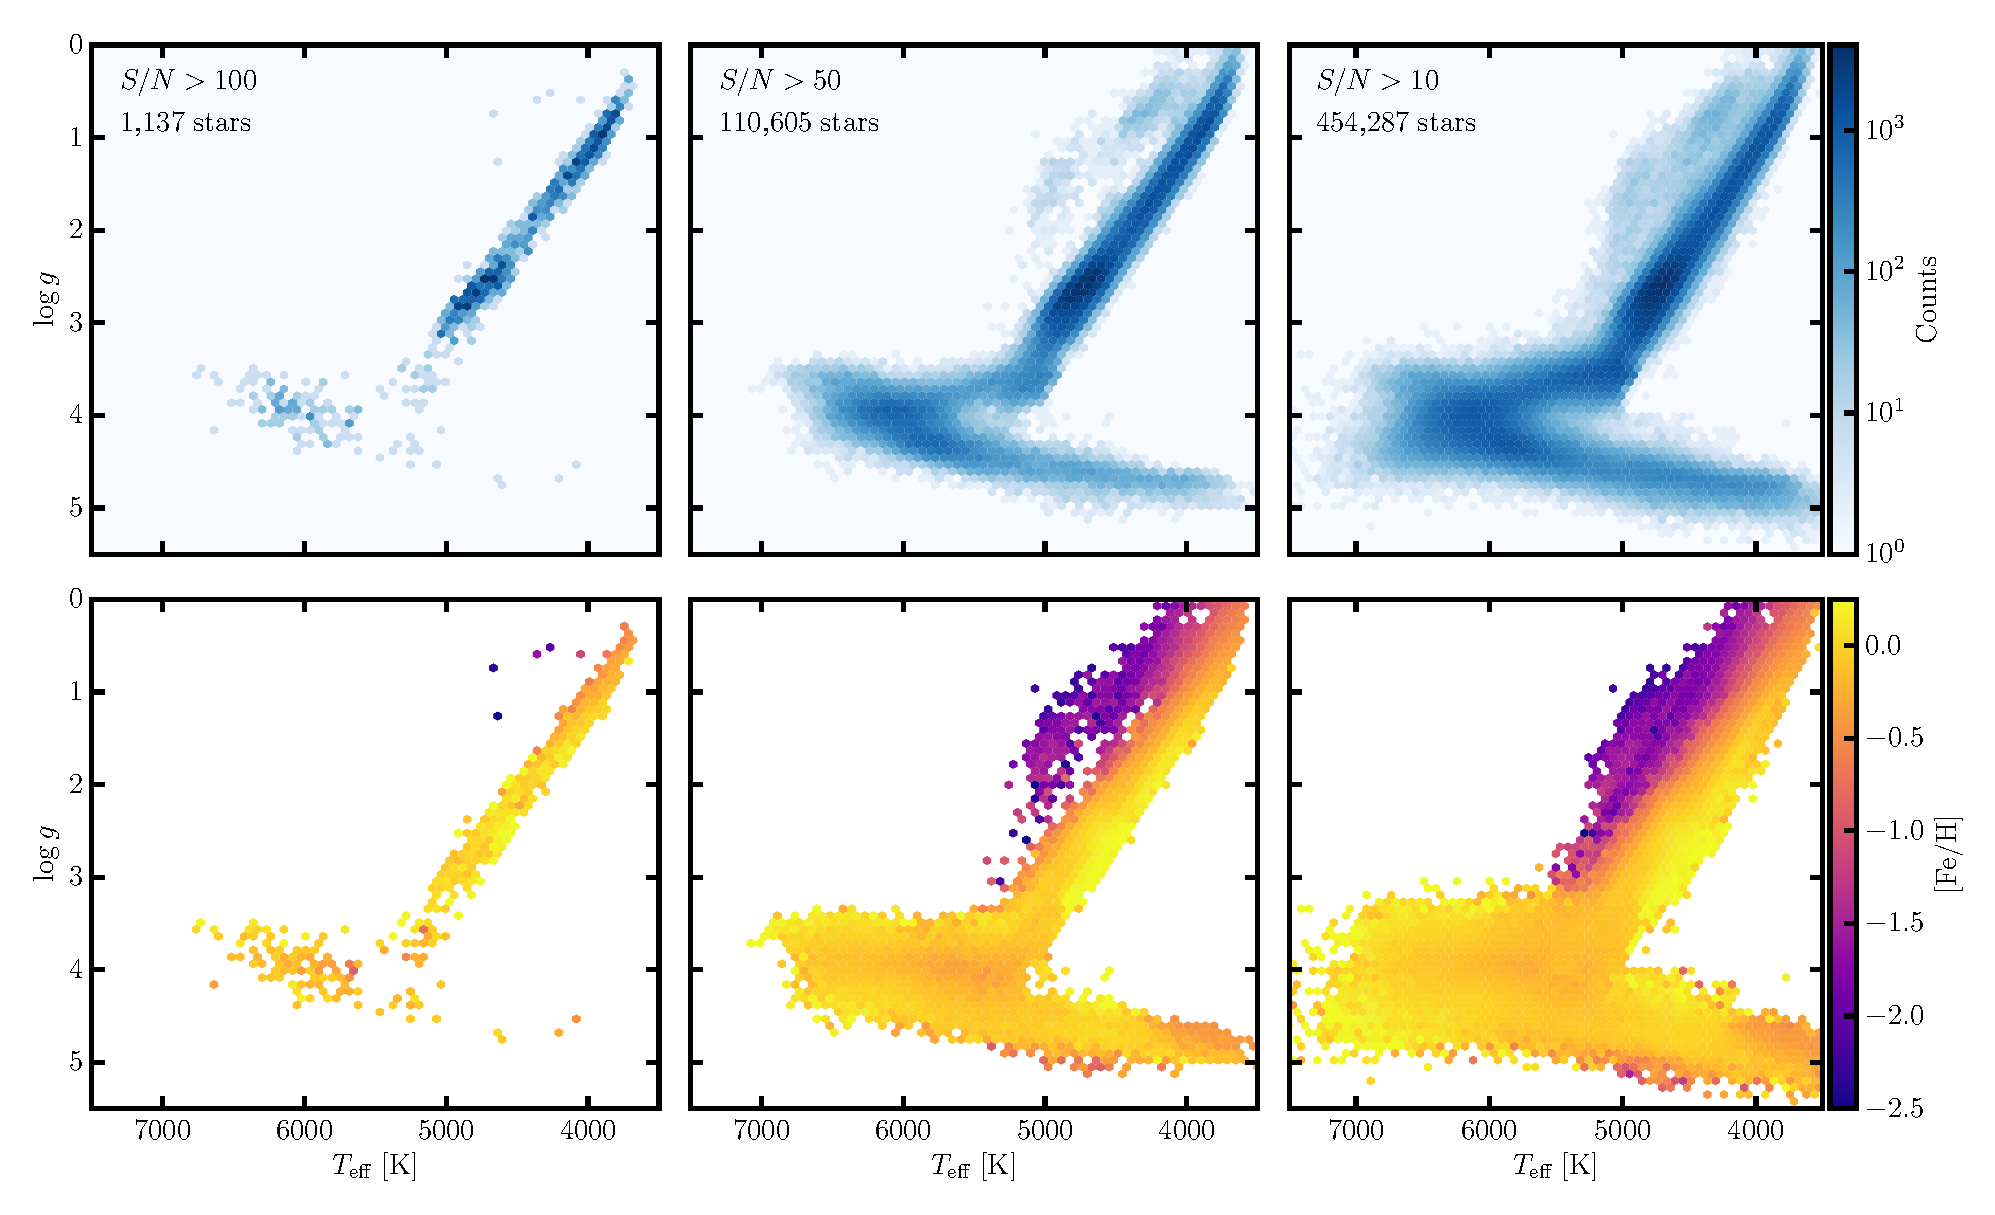
\includegraphics[width=\textwidth]{figures/hrd-test-set.pdf}
\caption{A `spectroscopic' Hertzsprung-Russell diagram showing the effective temperature $\teff$ and surface gravity $\logg$ for stars in the test set.  Only stars with $\chi_r < 3$ are shown, and each panel shows stars that meet a threshold in $S/N$ ratio.\label{fig:test-set-hrd}}
\end{figure}

\begin{figure*}[p]
\caption{The RMS of the test set labels as a function of S/N ratio for repeated stars in the test set.\label{fig:test-set-repeats}}
\end{figure*}

\begin{figure*}[p]
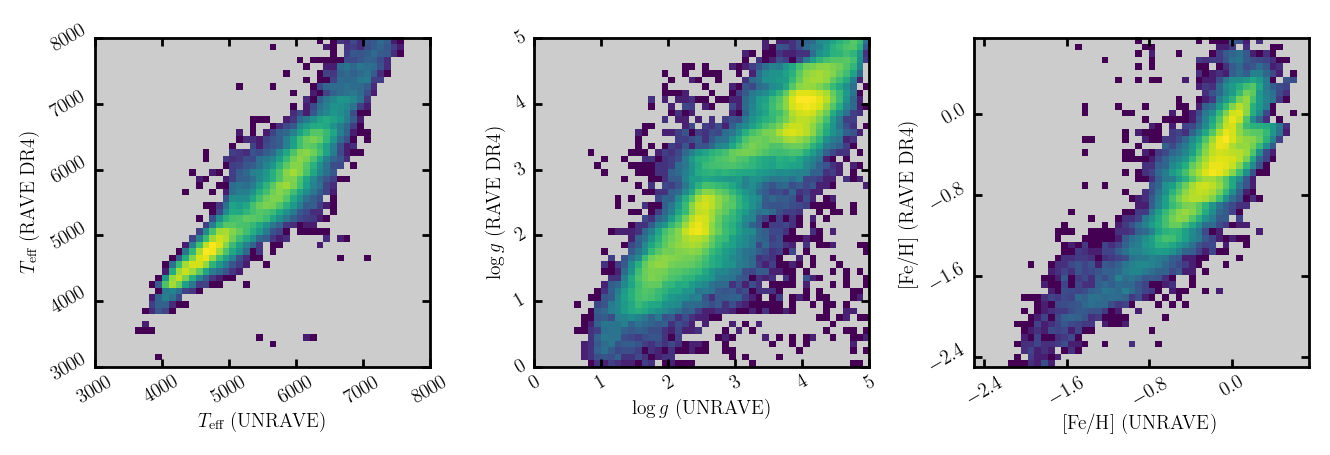
\includegraphics[width=\textwidth]{figures/dr4-comparison.png}
\caption{Stellar label comparison between the \project{UNRAVE} catalog and the \project{RAVE} fourth data release \citep{Kordopatis_2013}.\label{fig:rave-dr4-comparison}}
\end{figure*}


\begin{figure*}[p]
\caption{Stellar label comparison between the \project{UNRAVE} catalog and the \project{RAVE} fifth data release \citep{Kunder_2016}.\label{fig:rave-dr5-comparison}}
\end{figure*}

\begin{figure*}[p]
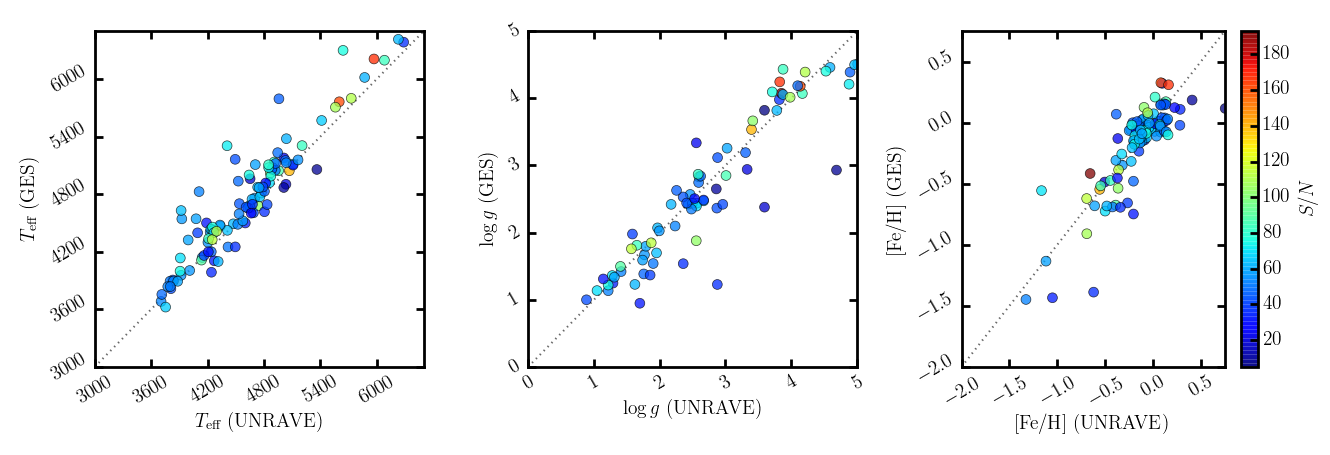
\includegraphics[width=\textwidth]{figures/ges-comparison.png}
\caption{Stellar label comparison between the \project{UNRAVE} catalog and the \project{Gaia-ESO Survey} fourth internal data release.\label{fig:ges-dr4-comparison}}
\end{figure*}

\begin{figure*}[p]
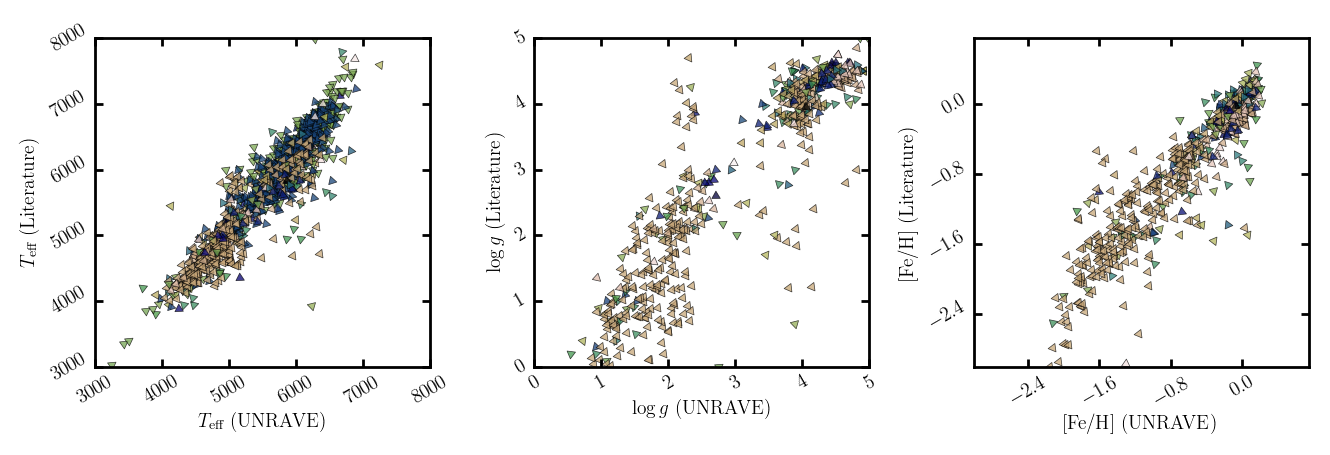
\includegraphics[width=\textwidth]{figures/literature-comparison.png}
\caption{Stellar label comparisons between the \project{UNRAVE} catalog and the samples discussed in \citep{Kordopatis_2013}}
\end{figure*}

\end{document}
